\documentclass[11pt,a4paper,twoside,openright,bachelor,english]{netthesis}
\usepackage[utf8]{inputenc}
\usepackage[section]{placeins}
\usepackage{float}
% Include common packages
% raise package limit
\usepackage{etex}

% input encoding
\usepackage[utf8]{inputenc}

% subfiles
\usepackage{subfiles}
\makeatletter
\newif\ifsubfile\subfilefalse
\@ifclassloaded{subfiles}{\subfiletrue}{\subfilefalse}
\makeatother

% fonts
\usepackage[T1]{fontenc}
\usepackage{libertine}
\usepackage[scaled=0.8]{beramono}
\usepackage[expansion,protrusion,shrink=15,stretch=15]{microtype}
% Use libertine symbols --- Dirty hack!
% Does no longer work with new libertine package
%\DeclareTextCommand{\textbullet}{T1}{\libertineGlyph{bullet}}
%\DeclareTextCommand{\textdagger}{T1}{\libertineGlyph{dagger}}
%\DeclareTextCommand{\textdaggerdbl}{T1}{\libertineGlyph{daggerdbl}}
%\DeclareTextCommand{\textasteriskcentered}{T1}{\libertineGlyph{asteriskmath}}
% Alternatively use cmsy but get rid of warnings --- Dirty hack!
%\DeclareTextCommand{\textbullet}{T1}{$\bullet$}
%\DeclareTextCommand{\textdagger}{T1}{$\dagger$}
%\DeclareTextCommand{\textdaggerdbl}{T1}{$\ddagger$}
%\DeclareTextCommand{\textasteriskcentered}{T1}{$\ast$}

% vim: set sw=4 ts=4 et tw=0 :



% tables
\usepackage{array}
\usepackage{booktabs}
\usepackage{tabularx}
\usepackage{longtable}
\usepackage{ltxtable}

% lists etc
\usepackage{cite}

% text configurations not including font
%% define a long dash
\newcommand\drule{\rule[.56ex]{\widthof{-}}{.1ex}}
\newcommand\nrule{\rule[.56ex]{\widthof{--}}{.1ex}}
\newcommand\mrule{\rule[.56ex]{\widthof{---}}{.1ex}}
\newcommand\lrule{\rule[.56ex]{1em}{.1ex}}

% reset some length
\setlength{\textfloatsep}{1.7\baselineskip plus 0.6\baselineskip minus 0.4\baselineskip}

% vim: set sw=4 ts=4 et tw=0 :



% math
\usepackage{mathtools}
\usepackage{packages/accents}
\usepackage{fixmath} % upper case Greek letters in italics.
% All mathematical definitions
% use msvsymbols package
%\usepackage{msvsymbols}

\usepackage[libertine,cmintegrals,libaltvw]{newtxmath}
\usepackage[
bb=ams,
scr=rsfs,
cal=cm
]{mathalfa}

% libertine math font stuff
\makeatletter
\DeclareMathSymbol{0}\mathalpha{operators}{"30}
\DeclareMathSymbol{1}\mathalpha{operators}{"31}
\DeclareMathSymbol{2}\mathalpha{operators}{"32}
\DeclareMathSymbol{3}\mathalpha{operators}{"33}
\DeclareMathSymbol{4}\mathalpha{operators}{"34}
\DeclareMathSymbol{5}\mathalpha{operators}{"35}
\DeclareMathSymbol{6}\mathalpha{operators}{"36}
\DeclareMathSymbol{7}\mathalpha{operators}{"37}
\DeclareMathSymbol{8}\mathalpha{operators}{"38}
\DeclareMathSymbol{9}\mathalpha{operators}{"39}
\makeatother

%% math alphabet fonts
\DeclareSymbolFont{nxlmibit}{OML}{nxlmi}{bx}{it}
\DeclareSymbolFontAlphabet{\mathbit}{nxlmibit}
%FIMXE: the first package seems to cause an \if\fi bug
%\DeclareSymbolFont{libertineplus}{T1}{ntxrx}{m}{n}
%\DeclareMathSymbol{+}{\mathbin}{libertineplus}{43}

\newcommand\showmathalphabet{\noindent\begin{tabular}{ll}
    mathnormal  & $abcdefghijklmnopqrstuvwxyz$\\
                & $ABCDEFGHIJKLMNOPQRSTUVWXYZ$\\
    mathrm      & $\mathrm{abcdefghijklmnopqrstuvwxyz}$\\
                & $\mathrm{ABCDEFGHIJKLMNOPQRSTUVWXYZ}$\\
%    mathit      & $\mathit{abcdefghijklmnopqrstuvwxyz}$\\
%                & $\mathit{ABCDEFGHIJKLMNOPQRSTUVWXYZ}$\\
    mathbf      & $\mathbf{abcdefghijklmnopqrstuvwxyz}$\\
                & $\mathbf{ABCDEFGHIJKLMNOPQRSTUVWXYZ}$\\
    mathbit     & $\mathbit{abcdefghijklmnopqrstuvwxyz}$\\
                & $\mathbit{ABCDEFGHIJKLMNOPQRSTUVWXYZ}$\\
%    mathfrak    & $\mathfrak{abcdefghijklmnopqrstuvwxyz}$\\
%                & $\mathfrak{ABCDEFGHIJKLMNOPQRSTUVWXYZ}$\\
    mathcal     & $\mathcal{ABCDEFGHIJKLMNOPQRSTUVWXYZ}$\\
%    mathscr     & $\mathscr{ABCDEFGHIJKLMNOPQRSTUVWXYZ}$\\
%    matheus     & $\matheus{ABCDEFGHIJKLMNOPQRSTUVWXYZ}$\\
\end{tabular}}

% vim: set sw=4 ts=4 et tw=0 :



% theorems
%% theorems and proofs
\newtheoremstyle{reportitalic}%
    {2ex}{2ex}{\normalfont\renewcommand\em\upshape\itshape}{}%
    {\normalfont\scshape}{.}{1em}{}
\newtheoremstyle{reportnormal}%
    {2ex}{2ex}{\normalfont}{}%
    {\normalfont\scshape}{.}{1em}{}
\theoremstyle{reportitalic}
\newtheorem{definition}{Definition}[chapter]
\newtheorem{theorem}{Theorem}[chapter]
\newtheorem{proposition}[theorem]{Proposition}
\newtheorem{corollary}[theorem]{Corollary}
\newtheorem{lemma}[theorem]{Lemma}
\theoremstyle{reportnormal}
\newtheorem{example}{Example}[chapter]
\newtheorem{remark}{Remark}[chapter]

% theorem enumerates
\newenvironment{thmenum}{\begin{enumerate}
    \setlength\itemsep{.2ex}
    \setlength\parsep{0pt}
    \setlength\parskip{0pt}
    \renewcommand\theenumi{\alph{enumi}}
    \renewcommand\labelenumi{(\theenumi)}
    \vskip -\topsep\vskip .2ex\vskip 0pt
}{\end{enumerate}}

% proof reference of theorem enumerates
\newcommand\proofrefskip{\hskip 1em\relax}
\newcommand\proofref[1]{(\ref{#1})}

% vim: set sw=4 ts=4 et tw=0 :



% listings
\usepackage{listings}

% drawing and graphics
\usepackage{packages/tumcolors}
\usepackage{tikz}
\usetikzlibrary{calc,arrows,matrix,positioning,shapes.multipart,shapes.geometric}

% commutative diagram
\tikzstyle{commutative diagram}=[matrix of math nodes,
    matrix anchor=m-1-1.base,anchor=base,
    row sep=3em,column sep=4em,
    minimum width=3em,minimum height=2em]
\tikzstyle{commutative edge}=[]
\tikzstyle{map}=[commutative edge,->]
\tikzstyle{injective map}=[commutative edge,right hook->]
\tikzstyle{surjective map}=[commutative edge,->>]
\tikzstyle{bijective map}=[commutative edge,right hook->>]

% broadcast diagrams
\tikzstyle{wireless}=[draw,thick,circle,
    minimum size=5.5mm,inner sep=0mm,font=\small]
\tikzstyle{virtual}=[draw,thick,rectangle,
    minimum size=5.5mm,inner sep=0mm,font=\small]
\tikzstyle{arc}=[draw,thick,->]
\tikzstyle{rate}=[pos=.5,above,sloped,font=\small]
\tikzstyle{broadcast}=[draw,thin,dashed]
\tikzstyle{broadcast rate}=[font=\small]
\tikzstyle{cut}=[draw,thick]

% Markov chains
\newcommand\clamp[1]{\raisebox{0pt}[0pt][0pt]{\makebox[0pt][c]{#1}}}
\newcommand\clampwd[1]{\raisebox{0pt}[\height][0pt]{\makebox[0pt][c]{#1}}}
\newcommand\clamphd[1]{\raisebox{0pt}[0pt][0pt]{\makebox[\width][c]{#1}}}

% vim: set sw=4 ts=4 et tw=0 :


\usepackage{packages/moeptikz}

% IEEE tools for tweaking bib style
\usepackage{packages/IEEEtrantools}

% enable links
\usepackage[colorlinks=false,pdfborder={0 0 0}]{hyperref}
\newcommand\toc{\relax}

% pgfplots
\usepackage{pgfplots}
\pgfplotsset{compat=newest}
\pgfplotsset{colormap={moepcolormap}{[1cm] color(0cm)=(black!60) color(5cm)=(black!1)}}
%\pgfplotsset{colormap={moepcolormap}{[1cm] color(0cm)=(TUMDarkerBlue) color(1cm)=(TUMLighterBlue) color(2cm)=(TUMGreen) color(3cm)=(TUMBeamerYellow) color(4cm)=(TUMOrange) color(5cm)=(I8LogoRed)}}



% Maybe we want to inlcude some additional packages


% hyphenation
\hyphenation{op-ti-cal net-work net-works semi-con-duc-tor tech-nique tech-niques}


% Needed for Bachelor's theses, Master's theses and IDP
\titlegerman{Leistungsanalyse der Funktionen von Middleboxes}
\titleenglish{Performance Analysis of Middlebox Functionality}
\submitteddate{\today}
\author{Simon Sternsdorf}
\supervisor{\NEThead}
\advisor{Florian Wohlfart}

% Additionally needed for dissertations
\committeechair{}
\committeeexaminers{}{}{}
\accepteddate{}


\begin{document}%

% Makes sure that same author names are not replaced by dahes
\bstctlcite{IEEEexample:BSTcontrol}

\pagenumbering{gobble}
\maketitle%


\subfile{include/abstract.tex}


\pagenumbering{Roman}%

{\tableofcontents}
{\listoffigures}
{\listoftables}

\cleardoublepage

\pagenumbering{arabic}

\chapter{Introduction}

\section{Motivation}
Middleboxes are mediating devices used by both End-user Internet Service Providers and normal home users. The requirements ISPs have for Middleboxes are of course vastly different from the requirements of private users. Thus the implementations differs greatly as well. Middleboxes for home users do not have high performance requirements. They conduct mostly very simple tasks for a low amount of devices. This is changing of course, as more and more web-enabled devices are used in modern households. 
Still the required performance is low in contrast to at an ISP for example. Especially carrier grade network address translation is used to provide ipv4 connectivity for mobile phones, since IPv4 addresses are getting rare \cite{A10}. The Middleboxes used are mostly implemented in hardware, which has assets and drawbacks. Those drawbacks are significant. 
Middleboxes specifically produced for ISPs are expensiv both in acquisition and maintainance, also they usually have to be replaced to introduce new features \cite{WhiteP}. Also they are difficult to scale with higher or lower demand. All these problems are avoidable through network function virtualization. And the long-term plan is indeed to replace these hardware middleboxes with all-purpose hardware that is cheap and easily replaceable \cite{Click}. The networking functions would be implemented in software. 7 of the worlds largest telecoms network operators are in an standards group for virtualization of network functions. So the topic is already being discussed in ISPs \cite{NetDis} 



\section{Goal of the thesis}
The goal of this thesis is to test different software Middlebox implementations. We will install different middlebox implementations in our testbed. Then we will test the packet processing capability, try to find bottlenecks for the performance when processing packets. We will evaluate our results. 
Additionally we want to evaluate if software Middleboxes are competitive with hardware implemented Middleboxes and could replace them in the foreseeable future. 

\section{Outline}

The thesis reads as follows. The second chapter introduces the theoretical concept of NAT and a NAT model which we used in our tests. Also it defines performance testing. Additionally the Data Plane Development Kit is introduced, DPDK. The third chapter informs the reader about the general idea behind our tests. Further it presents the software used for the tests. This includes the software running on the device under test, as well as the software used to run the tests. It explains the methodological approach used in this thesis. Here it explains the setup for the experiment. In chapter 4 are the collected results of the Firewall and NAT tests with a brief analysis of the result. Finally chapter 5 summarizes the outcome and gives possible future works of this thesis. 

\chapter{Background}

This chapter gives a overview over network address translation and the NAT model we will assume in this thesis. Also it will explain our approach to performance testing. Finally the chapter outlines the Data Plane Development Kit, developed by Intel \cite{DPDKOv}.

\section{NAT}

Network address translation NAT was first described 1993 and written into RFC 3022 \cite{RFC3022} in 2001. It was proposed as an temporary solution for the shortage of IPv4 addresses. It should slow down the need for IPv4 addresses of private customers and businesses \cite{bonaventure2011computer}. It does this by working as a connector between two different networks with different IPv4 address spaces. Mostly it translates between the address space of the Internet and a private network. Since NAT is used so broadly it is one of the most common middleboxes. $\newline$
NAT in private households is in many instances implemented directly in the router. The home ususally only gets one IPv4 address from its ISP. The router then interconnects the home network to the Internet via an ISP. It translates the private IP addresses of the home network to enable them to share the single IPv4 address \cite{bonaventure2011computer}[Page 168]. In corporate networks it basically fulfills the same purpose. The main difference is that the border router manages multiple public IPv4 addresses and manages the correct translation between them and the private IPv4 addresses in the private network. 
Here we see the simple version with only one public IPv4 address.

\begin{figure}[h]
\centering
{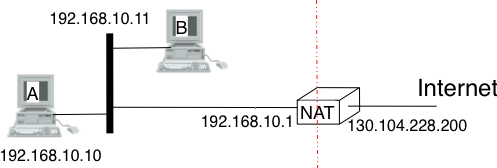
\includegraphics[width=.75\columnwidth]{figures/NATPrivate}} \quad
\caption[A simple NAT with one public IPv4 address]{ A simple NAT with one public IPv4 address \cite{bonaventure2011computer}[Page 168]}
\label{fig:NATPrivate}
\end{figure}

A NAT middlebox manages the translation between the different IPv4 address spaces. To achieve this the middlebox has to save a mapping of the private IP addresses to the public ones. In the simplest imaginable case we have as many public IPv4 addresses as we have private ones. In that case the mapping is simply a bijection. When the NAT middlebox receives a packet from a new private IP S in the internal network it maps it to a not used public IP from its address pool. This mapping is saved. To translate the packet the NAT middlebox has to : $\newline$
\begin{enumerate}

\item Replace the original source IP from the packet with the mapped public IP
\item Completely recompute the IP header checksum, as not only the Time To Live header field changes, but also the source IP header field \cite{tanenbaum1996computer}[Page 435]
\item Recompute the checksum in the TCP or UDP header if existent. The checksum of these protocols computes the checksum over the whole packet

\end{enumerate} 

When an answer from the Internet arrives the NAT middlebox has to to the same process only with replacing the destination IP address with the source address of the private host. This is done with the same mapping. Afterwards the packet is forwarded to the host in the private network. $\newline$
In the realistic case where we have less public IP addresses then private ones the translation occurs over the IP and the port number. An NAT middlebox that uses this translation method maps the internal IP and the internally used port number of the TCP or UDP packet to a public IP from the IP pool available to the NAT middlebox and the first available port number \cite{bonaventure2011computer}[Page 169]. The entries in the mapping table are removed by the system after either the TCP connection is closed or the connection is idle for a longer time. Here the NAT middlebox functions similarly to a stateful firewall, which will become important later. 
When the NAT middlebox has to handle packets from the Internet, it looks up a mapping from its state table for the destination IP address and the destination port. If a matching mapping exists the packet is translated accordingly and forwarded to the matching internal host. If no such mapping exists the packet gets discarded, as there is no way to determine the correct internal host. $\newline$
NAT has two main disadvantages: Opening TCP connections from the Internet to an internal network is very difficult. This means that for example FTP users behind NAT have problems. In active mode, the FTP client first establishes a control connection to the server.After that the client listens on a random port for the incoming data connection from the server. If the client sits behind a NAT this connection will not work \cite{FTP}.$\newline$
The other disadvantage is that NAT breaks the end- to end transparency of the IP layer and the application layer. This problem occurs when the IP address is used in the application layer, as the NAT only replaces the IP in the IP header. This can be avoided with an Application Level Gateway installed at the NAT. However it is not feasible to install an an ALG for every application that relies on the IP in layer 7 \cite{bonaventure2011computer}[Page 169]. $\newline$
IPv6 would make NAT middleboxes obsolete, although some people argue NAT still has some use cases when only IPv6 is used. This is discussed in RFC 5902 \cite{RFC5902}. With IPv6 enough addresses are available to give each device a unique global IP. 

\section{NAT model} \label{NATmodel}

This section is about the NAT model we will use in this thesis and why it is important for the performance tests we did. This model is based on the basic concept of how a NAT middlebox works. Roughly speaking we will split up NAT in different components. This way we can get an better understanding of which part of the NAT is actually responsible for how much of the time we need to forward a packet. $\newline$ 
In the model the NAT middlebox performs 3 tasks excluding the sheer forwarding of the packet: 
\begin{itemize}
\item Parse the packet. This means it has to check the IP header for the source  and destination IP address and also the port numbers. Here the NAT compares to a stateless firewall, which has to do the same things. 
\item Holding a state. The NAT middlebox has to remember the mapping it created for a connection. This is similar to the state-holding of a stateful firewall. A stateful firewall tracks the state of every single TCP connection that goes through it and keeps a 5-tuple for every open connection. This 5-tuple persists of the source and destination IP, the source and destination port and the protocol used for the connection. This makes 5-tuple unique to its connection \cite{bonaventure2011computer}[Page 167].
\item Rewriting either the source or destination IP address, and rewriting the source or destination port respectively. When the NAT middlebox has to translate the packet to forward it either to the Internet or the private network it has to replace the right IP address and the right port. 
\end{itemize}
$\newline$
This simple model for a NAT middlebox will us help hopefully to determinate the different factors that influence the performance of the NAT middlebox.  


\section{Performance testing}

Performance testing is the term that designates a testing technique to determine how a system reacts in term of steadiness and amenability under different amounts of load. 
With this testing we can learn about the quality of our system and its attributes \cite{TutPer}. There are different forms of performance testing. $\newline$
\begin{itemize}

\item Load testing. Load testing is a very simple form of performance testing where the system is tested under specific work loads. All the parts of the system get monitored. With this one can predict how the system will react in the future under concrete work loads.

\item Soak testing. Here the system is monitored under an continuous load. The load is set to the excepted average work load the system has to handle. With this testing the endurance of the system is determined. Critical parts like the memory of the system are monitored to find possible performance issues or errors under uninterrupted use.

\item Spike testing. As the name suggests this testing revolves around a sudden spike of new users in the system. This is simulated by suddenly increasing the number of virtual users and monitoring the system. This test shows if a system can manage such a strong spike of new users and also if the system can handle the continuous workload that comes with a bigger user base.

\item Stress testing. Stress testing is used to determine the maximum workload a system can handle. Also it shows how a system performs with a workload well above its limits. This is done by monitoring the system and increasing the workload until a part of the system fails or cannot complete the work correctly.

\end{itemize}
$\newline$

We will take a closer look at stress testing since it is the main form of performance testing we used here. In a stress test the condition of our system is progressively worsened until the performance is too low as that we could use the system or the system fails entirely. To exactly determine which element of the system failed we have to have indivisual stressors that are varied, and see which effect they have. Stress testing can often take a long time, but is really important to determine the degree of graceful degradation of a system. Graceful degradation describes the capability of a system to still be somewhat operational even under extreme circumstances. This is important for critical systems which always have to be operational \cite{Stress}. 



\section{Data Plane Development Kit}

The Intel Data Plane Development Kit, Intel DPDK, is a group of programming libraries available in source code. These libraries enable faster basic data plane functions on Intel processors. These lbraries are especially designed to optimize the packet processing capabilities on IA processors. These are processors from the Xeon series. These libraries allow for fast implementation of packet forwarding functions \cite{DPDKEx}.
The most important DPDK elements can be seen in \ref{fig:DPDKEx} 
\begin{figure}[h]
\centering
{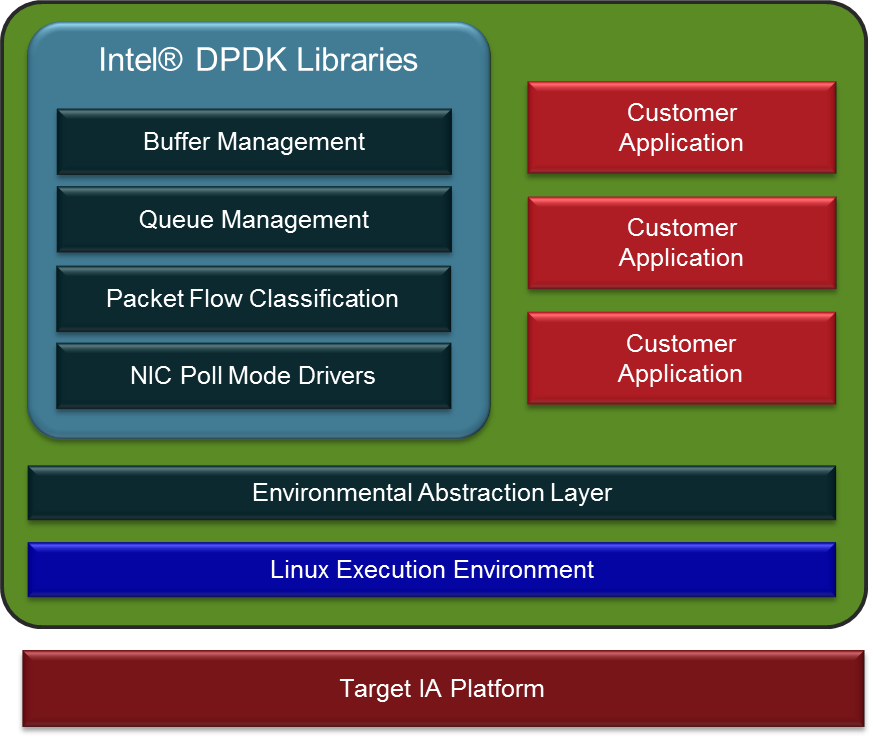
\includegraphics[width=.75\columnwidth]{figures/IntelDPDK}} \quad
\caption[ Intel® Data Plane Development Kit]{ Intel® Data Plane Development Kit \cite{DPDKEx}}
\label{fig:DPDKEx}
\end{figure}

This shows the different DPDK libraries for buffer management, queue management, packet flow classification and poll mode drivers for different network interface cards. DPDK provides a model with a low overhead to enable a optimal data plane performance. It includes an Environment Abstraction Layer, which includes platform specific code. This simplifies application porting \cite{DPDKEx}. $\newline$
The buffer management includes the DPDK Memory Manager, which allocates pools of objects in the memory. This is realized through a ring to store free objects, which accelerates the whole process. Additionally the DPDK Buffer Manager reserves buffers with a fixed size. This additionally accelerates the system, as we no longer have to constantly allocate new buffers or free buffers which are no longer in use. $\newline$
The packet flow classification includes the Intel DPDK Flow Classifier, which uses Streaming SIMD Extensions to speed up the process of placing packets in the right flow to get them processed. This additionally improves the throughput of the system \cite{DPDKEx}.
$\newline$
The poll drivers included in DPDK work for Gigabit Ethernet and 10 Gigabit Ethernet and work with asynchronous signal mechanisms. This improves the performance for pipe-lining packets. $\newline$
Since 2013 exists dpdk.org \cite{DPDKOv}, a Open Source Project founded by 6WIND \cite{DPDKEx}. Through this project source code, a documentation and example applications are available. This code is pretty much up-to date with the Intel DPDK releases and provides high processing-performance. The open-source project sees a lot of interest and is used already in several big projects and of course many smaller programs. One of them is for example MoonGen, which we will discuss in the Methodology chapter. $\newline$ 
As a short conclusion in DPDK, we can see that DPDK could be vital to accelerate packet processing and handling in software middleboxes. It has great capabilities and sees a lot of ongoing development from Intel \cite{DPDKEx}.


\chapter{Methodology}

Before we can start testing the performance of a software middlebox of our choice, we have to decide on test parameters. This involves how we should conduct the measurements, what we want to measure, how the measurements should look like etc. For example we have to decide on a load generator, what kind of test environment, how we want to collect and visualize the data that we derive, and most importantly the middlebox software we want to survey. 
$\newline$
In this chapter we talk about the research methodology and how to build it \cite{schmidt2017}[Page 23].

\section{General Idea}

To test a software middlebox we defined a specific test setup which will help us derive the most precise results. This means we will be able to determine in which areas the middlebox software is performant and which properties of our traffic are most influential on this performance. The exact setup will be described in the following section. $\newline$
The short abstract of it is: We will conduct black box tests of a middlebox software we installed on the DUT, the device under test. This DUT is connected to our testserver. This testserver runs a load generator to stress test our middlebox software. $\newline$

\begin{figure}[H]
\centering
{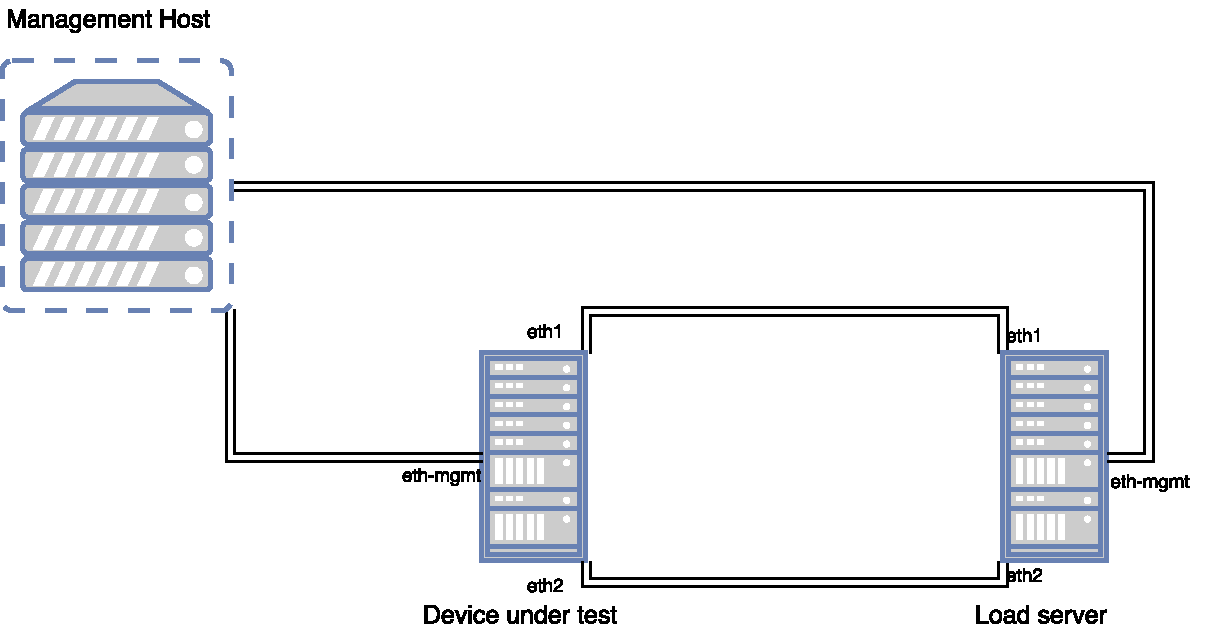
\includegraphics[width=.85\columnwidth]{figures/Testsetup}} \quad
\caption[Our testsetup ]{ Testsetup }
\label{fig:Testsetup}
\end{figure}
$\newline$

\subsection{Black box testing}

Black box testing is an important part of testing software. It it's core it is used to analyze software without knowledge or reference to the internal working of the software. This enables us to test the functionality of the software with basically no consideration of the internal processes of the software \cite{khan2010different}. 

\begin{figure}[H]
\centering
{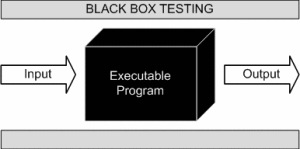
\includegraphics[width=.65\columnwidth]{figures/black_box_testing}} \quad
\caption[Working process of Black box testing ]{Working process of Black box testing \cite{BlackboxWiki}}
\label{fig:BlackBox}
\end{figure}

$\newline$
This method has following advantages for the tester:
\begin{itemize}

\item The tester does not need to know how the software that they test is implemented. This means the tester does not have to be a software developer. 

\item The tester can be someone independent from the developer, removing possible bias from the tests and how the are conducted. This means there exists no "bond" between the tester and the code. 

\item The perception for the tester is very simple

\end{itemize} 

Some disadvantages of blackbox testing for our case include: 
\begin{itemize}

\item Not all the possible inputs can be tested. This means for the middlebox for example, we can't test every single possible combination of flow length, packet size and transmit rate.

\item When tests throw errors it is harder to understand and determine why this certain test failed, as we can't just look inside the running DUT.\cite{khan2010different}

\end{itemize}



\subsection{Software}

For the tests we need software to implement and run the DUT and software to generate and record traffic. For one we need the middlebox software. As explaned in \ref{NATmodel} we want to implement and understand NAT in different states. This means our software middlebox needs to be very flexible. As our main features we need a stateless firewall and the NAT functionality. The software needs to run on our hardware under Linux. Preferably the software should use DPDK or similar software to increase the performance of the packet forwarding. Otherwise if the software uses the Linux Kernel it should at least have the option to use DPDK in the future. To test the performance of the DUT we need a load generator. The load generator needs to generate enough load to saturate a 10 gigabit Ethernet connection, as our two servers are connected with 10 gigabit Ethernet. Technically the load generator only needs to generate more load than the DUT can handle. As we do not know how much middlebox software on our server can handle we try to shoot for the maximum load possible. Also our load generator must be able to accurately measure the latency of our packets. Important for the tests are the different metrics we can define with the load generator. To fully test the middlebox we need to be able to change the metrics of our packet stream very freely. This includes the packet sizes, different ports, different IP addresses and different transmit rates.

%%Potential: Testframework


\section{Test Methodology}

This section introduces the specific software we chose for the testsetup. We will discuss the advantages and disadvantages of the choices we made. Also we will explain the experimental setup we arranged to test the middlebox software. A great deal of the setup was already established by the testbed. 


\subsection{Experimental Setup}

For the conducted experiments I used mostly the 2 same servers. When unavailable I used different servers in the testbed, but the servers have mostly the same hardware. 
$\newline$ 
The Hardware of one server was: 
\begin{itemize}

\item CPU: Intel(R) Xeon(R) CPU E31230 @ 3.20GHz

\item Number of CPUs: 1
\item Memory: 16 GB
\item Mainboard: X9SCL/X9SCM
\item NICs: 2x Intel X540 (1x X540-T2)


\end{itemize}

As operating system Debian 8.9 "Jessie" was used, as it was newest Debian system at the time. It was not further modified in any way. Debian was already preconfigured in the testbed for easy install. By using Debian I was able to automate most of the setup process for the device under test and the load server. The servers were connected as can be seen in \ref{fig:Testsetup} with 10 Gbit cables between them. On one server I installed the load generator on the other on the middlebox software which I configured for the tests. The following sections will explain the used programs in more detail. 

\subsection{MoonGen Traffic Generator}

\subsubsection{Advantages and disadvantages}

MoonGen is a traffic generator that can saturate 10 Gbit Ethernet easily while using a very special approach for measuring the latency of the packets. MoonGen was selected out of a few possible candidates mainly because of its flexibility. Most packet generators are either very complicated or have no good performance. The tested alternatives to MoonGen were either very complicated to set up and run, or had a bad performance \cite{emmerich2015moongen}. MoonGen has 4 major advantages over the rest for my use case: $\newline$
\begin{itemize}

\item MoonGen is completely implemented in software and can run on a lot of commodity CPUs. This is achieved through its implementation on top of DPDK, the packet processing framework. The only requirement for our hardware is that DPDK supports it and that it offers support for the time stamping and rate control. 

\item Is very flexible, as the packet generator logic is written in Lua scripts. These scripts are very user friendly and can be completely modified. In this specific case LUA-JIT was used as its performance is suited for high speed packet processing. 

\item Is able to saturate multiple 10 Gbit Ethernet interfaces with minimum size packets. This advantage was not really necessary for this specific test setup as we only needed to saturate on interface. But the good performance was still noticeable. 

\item MoonGen allows to time stamp very accurately and building on that very good rate control. This point will be further explained below. 

\end{itemize}

One disadvantage of MoonGen is that it currently only supports UDP packets for layer 3 latency measurements. MoonGen is not able to understand the TCP stack and therefor cannot establish a TCP connection. This was important when testing the middlebox software mOS, which will be talked about later. 

\subsubsection{Closer Look: Hardware timestamping }

The type of hardware timestamping in MoonGen is very unique. It utilities the IEEE 1588 Precision Time Protocol (PTP), which is used for clock synchronization across networks. It is supported by a large variety of NICs. PTP is either used as a protocol on layer 3 or on top of UDP on layer 4. This hardware timestamping works at the moment Intel 82580 GbE, the 82599 and X540 10 GbE chips. These NICs support the timestamping with PTP Ethernet and UDP. Moongen configures them to only recognize PTP packets with a specific first byte in their header. The second byte represents the PTP version number. The other PTP fields are not used and can contain any value. This allows MoonGen to measure the latency of any packet. All timestamps fro recieved and transmitted packets get saved in a special register directliy on the NIC. This register has to be read out before the next packet can be timestamped. Some NICs also support the prepending of timestamps of new packets to the buffer. With these timestamping mechanisms MoonGen can reach a precision of 64 nanoseconds on a 10GbE link \cite{emmerich2015moongen}.


\subsection{mOS}
This section will explain why mOS was chosen initially as a middlebox candidate and why it wasn't usable for this paper. $\newline \newline$

\subsubsection{Approach of mOS}
Middlebox OS is a reusable networking stack, which enables stateful flow processing. mOS provides an API for developers to programm middlebox applications on top of mOS. This enables the developers to concentrate on the important logic of the middlebox and the top level rather than the finicky low-level packet processing. This means the applications would be more consistent and easier modifiable. Also it prevents the introduction of new errors when the programmer has to implement the complex flow mechanisms from scratch. Most importantly, mOS promised a consistent and high performance even though it essentially provides a software middlebox. The developers of mOS promised an "effizient event system that scales to monitoring millions of concurrent flow events" \cite{jamshed2017mos}[Abstract]. $\newline$
The API of mOS includes programming presets that introduce the programmer to flow-events. Flow-events are operations the middlebox can fulfill which are definable by the user. This makes mOS very easy to deploy and to adjust to your networking situation. 

\begin{figure}[H]
\centering
{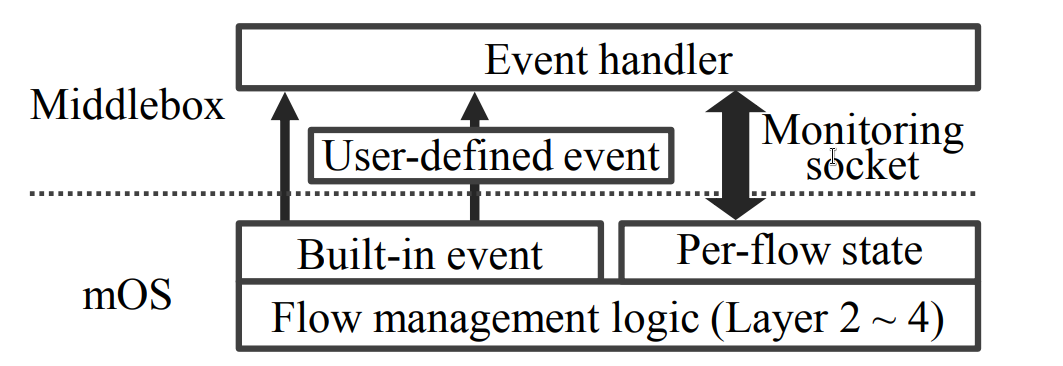
\includegraphics[width=.85\columnwidth]{figures/mOSFlow}} \quad
\caption[ mOS/Application Interaction]{ mOS/Application Interaction \cite{jamshed2017mos}  }
\label{fig:mOSFlow}
\end{figure}

$\newline$
mOS enables easier development by providing a monitoring socket for developers. This enables the developer to see exactly what happens with a single TCP flow running through the middlebox. Additionally, mOS includes scalable monitoring. Scalable monitoring helps to reduce the overhead that gets induced when tracking so many different flows. This reduces the memory usage of mOS for example for dynamic event registration and deregistration. Also developers can enable and disable event generation for flows and reduce recourse usage this way. By deacticating the tracking of unnessesary properties if the flows mOS reduces the overall system load. This leads to higher performance and reduces waste of CPU cycles \cite{jamshed2017mos}. $\newline$

\begin{figure}[H]
\centering
{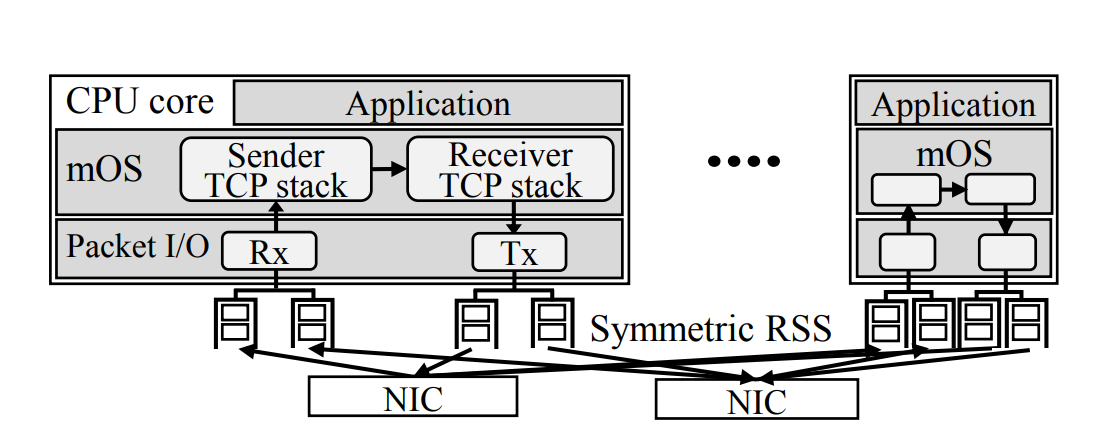
\includegraphics[width=.85\columnwidth]{figures/mOSThread}} \quad
\caption[ mOS application threading model]{ mOS application threading model \cite{jamshed2017mos}  }
\label{fig:mOSThread}
\end{figure}
$\newline$
To increase performance, mOS uses a shared-nothing parallel-processing threading model. This model works especially great on modern multi-core CPUs. As you can see in \ref{fig:mOSThread}, mOS initializes n threads each bound to a CPU core. Each of these threads handles flows using symmetric receive-side scaling (S-RSS). All packets that are associated to the same connection are mapped by S-RSS to the same RX queue in the NIC. This enables the forwarding of packets with line rate, as all the packet classification is done in hardware by the NIC itself which is very performant. This also enables the shared-nothing parallel-processing threading model, as every connection is handled by one thread. This enables mOS to avoid inter-clock locks and cache interferences \cite{jamshed2017mos}.   
$\newline$

mOS relies on kernel-level NIC drivers to forward the packets into the symmetric RSS. DPDK or PCAP are supported as default I/O module. $\newline$

\begin{figure}[H]
\centering
{\includegraphics[page=11,width=.65\columnwidth]{figures/mOSDPDKSummit}} \quad
\caption[ mOS shared-Nothing Parallel Architecture]{mOS shared-Nothing Parallel Architecture \cite{mOSStack}  }
\label{fig:mOSStack}
\end{figure}

Figure \ref{fig:mOSStack} displays the function of the NIC-drivers. mOS reads multiple packets at once from the incoming packet stream. 

$\newline$
We initially chose mOS as our middlebox test candidate because it promised great performance with high flexibility. Since it is based on mTCP it can work with the complete TCP stack and we planned to make further tests with the TCP stack. In its repository mOS also includes sample applications. These seemed very useful, as a NAT application and a stateless firewall application were given. With the simple expression language mOS uses for the applications they seemed easily modifiable. Also the testing of the sample applications could get us some insight in how the middlebox applications performed in our testbed with our load generator in general. mOS can run on commodity hardware. The hardware in our testbed is not exactly the same as the developers used in their paper but it is similar enough. 



\subsubsection{Setup in the testbed}

To set up the base mOS on one of the servers in the testbed I followed the documentation of the mOS developers. This involved installing several packages of the Debian repositories as well as installing DPDK with all its dependencies. We decided to use mOS compiled with the DPDK library and not with the PCAP library. We made this decision based on the data from the mOS developers, which promised a better performance with the DPDK libraries \cite{mOSStack}.


\subsubsection{Problems}

\subsection{Open VSwitch}

Open VSwitch is the middlebox software we settled on using. In it's core, OVS is a virtual switch. Hypervisors need to bridge traffic between VMs and the outside network interface. When the hypervisor is Linux-based this usually means using the standard Linux bridge, which is the L2-switch that is build into Linux. This switch is mostly fast and reliable, but has problems concerning multi-server virtualization. Here Open VSWitch provides to be more useful and performant than the Linux bridge. \cite{OpenVSwitchWhy} $\newline$ Open VSwitch is licensed under the Apache open source license. Open VSwitch supports most of the standard management interfaces and protocols. It works in the most commonly used virtualization environments like Xen, KVM and Virtualbox as well in virtual management systems. It is mostly used to virtualize multiple servers at once \cite{pothuraju2016measuring}. 
$\newline$
\begin{figure}[H]
\centering
{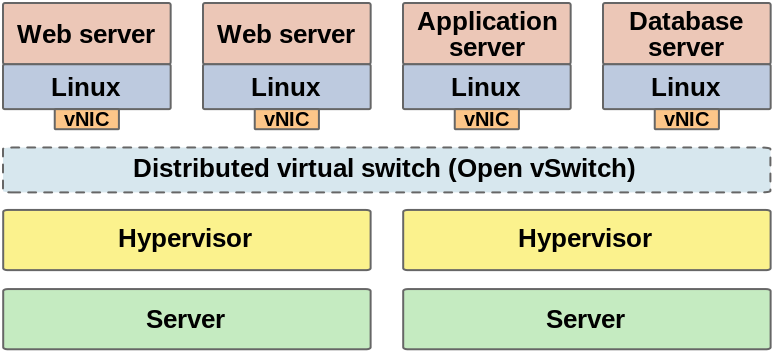
\includegraphics[width=.85\columnwidth]{figures/OpenVSwitch}} \quad
\caption[ Distributed OpenVSwitch ]{ Distributed OpenVSwitch \cite{OpenVSwitchNVFI}  }
\label{fig:OpenVSwitch}
\end{figure}

Open VSwitch enables logical abstraction between different virtual machines and handles the offloading to the actual switching hardware. To control this OVS lies on top of the virtualization layer of the hypervisor and provides interfaces to the virtual machines. $\newline$
The virtual machines contain virtual interfaces. These enable communication between the VMs running on the same hypervisor or connected in the same virtual network and forward the traffic to the actual network interface of the machine. Here OVS acts as a bridge between the VMs and the physical interfaces. In short it interconnects the virtual interfaces with the physical interfaces \cite{pothuraju2016measuring}. 

\subsubsection{Advantages of Open VSwitch}

Open VSwitch is used as an alternative to the basic Linux bridge for modern hypervisors. OVS has some clear cut advantages over the classic Linux bridge mostly in terms of performance. 
\begin{itemize}

\item Fast self-regulation when the network environment changes, realized through sFlow and Netflow. 

\item Very easy configuration and automation of network systems. Slow and fast network states can be migrated between instances. 

\item OVS can manipulate packets to enable a better administration of different flows. This means especially changing tags in packets or reordering them. This can speed up the network processes. \cite{pothuraju2016measuring}

\end{itemize}


\subsubsection{OVS with DPDK support}

Open VSwitch forwards packets over the kernel data path, which means it uses the standard Linux kernel. This method divides the packet processing in a slow path and a fast path. The fast path matches incoming packets on a flowtable to determine the forwarding rule for the specific packet. The first packet from a new flow does not match anything in the flow table and is sent via the slow path in the user space daemon. After the user space has processed the packet, the user space daemon gets the information for the flow table from him and includes them in the current flow table. All subsequent packets of the flow can be handled via the fast path again. $\newline$
By using this approach native OVS is a lot faster than normal user space packet forwarding. Still, the context switching required for new flows limits the realistically achievable throughput. This means native OVS is not feasible for use cases were a high throuhgput is mandatory \cite{OpenVSwitchDPDK}.  $\newline$
With the use of DPDK in OVS, the slow path can make use of the Poll Mode Drivers. These enable the fast forwarding of packets from the user space to the interfaces, without the need for extra interrupt handling of the kernel. This means we essentially bypassing the whole kernel network stack. By incorporating DPDK with the Poll Mode Driver in Open VSwitch the slow path essentially becomes the fast path, as in both cases the path of the packet is the same. $\newline$
\begin{figure}[H]
\centering
{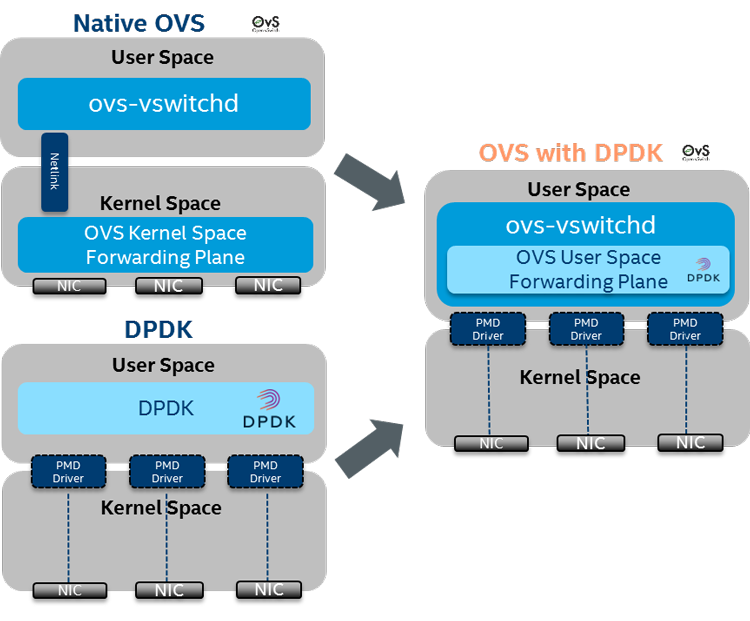
\includegraphics[width=.80\columnwidth]{figures/OVSDPDK}} \quad
\caption[ OpenVSwitch with and without DPDK]{OpenVSwitch with and without DPDK \cite{OpenVSwitchDPDK}  }
\label{fig:OpenVSwitchDPDK}
\end{figure}

This can be see in \ref{fig:OpenVSwitchDPDK}. Sadly the NAT extension of OVS does not support DPDK just yet. The support is announced for version 2.7 which will probably be released in 2018 \cite{OVSNATDPDK} . %%Possible Extension from Intel Page

\subsubsection{Connection tracking in OVS}
The connection tracking module in OVS is relatively new. Originally OVS only supported stateless matching.That made the implementation of firewalls quite difficult. For example does OVS support the match on TCP flags. This enables a fast stateless firewall by matching on TCP SYN and TYP ACK flags. But UDP traffic and traffic with ACK flag set gets through the firewall unhampered. Another way to set up a firewall in OVS is with a learn action which builds a new flow in the reverse direction. But this has to direct new flows once again through the user space which reduces the speed significantly \cite{OVSconntrack}. $\newline$
With OVS 2.5 a connection tracking module was introduced. It supports the stateful tracking of flows as well as application-level gateways for different protocols like ftp. 

\begin{figure}[H]
\centering
{\includegraphics[page=6,width=.90\columnwidth]{figures/OVSconntrack}} \quad
\caption[ OpenVSwitch with the conntrack module]{OpenVSwitch with the conntrack module \cite{OVSconntrack}  }
\label{fig:OpenVSwitchconntrack}
\end{figure}

As you can see in \ref{fig:OpenVSwitchconntrack} the new conntrack module allows us to create and update CT entry's without the need to go through the user space. This greatly improves the performance of the action. With the new module come different extensions for OpenFlow, which allow us to send a new connection to conntrack to start tracking it. The extension match on fields in the first packet. $\newline \newline$
This stateful matching enables a lot of other applications for OVS, for example also stateful NAT. As of now, OVS supports DNAT and SNAT. At the moment this uses the NAT features of netfilter, which is the packet filtering framework in Linux. With netfilter the OVS NAT supports port range and address range mappings with different mapping modes. 
This means the stateful NAT in OVS has all the features we expect from a middlebox NAT. 
\begin{figure}[H]
\centering
{\includegraphics[page=13,width=.90\columnwidth]{figures/OVSconntrack}} \quad
\caption[Stateful NAT flow in Open VSwitch]{Stateful NAT flow in Open VSwitch \cite{OVSconntrack}  }
\label{fig:OpenVSwitchNATflow}
\end{figure}

As you can see in \ref{fig:OpenVSwitchNATflow}, the conntrack and the NAT module in Open VSwitch use netfilter to create and update the rules. Created routes get stored in the OVS flow table. 

\chapter{Evaluation and Analysis of results}

\section{Firewall tests}

\section{NAT tests}

\chapter{Conclusion}

\section{Future Works}


%\subfile{include/outline.tex}
\appendix
%\subfile{Appendix.chap.tex}

%\subfile{Nomenclature.chap.tex}



\bibliographystyle{packages/IEEEtran}
\bibliography{lit}

\end{document}

% vim: set sw=4 ts=4 et tw=72 :

